\documentclass[11pt,a4paper]{report}
\usepackage[textwidth=37em,vmargin=30mm]{geometry}
\usepackage{calc,xunicode,amsmath,amssymb,paralist,enumitem,tabu,booktabs,datetime2,xeCJK,xeCJKfntef,listings}
\usepackage{tocloft,fancyhdr,tcolorbox,xcolor,graphicx,eso-pic,xltxtra,xelatexemoji}

\newcommand{\envyear}[0]{2025}
\newcommand{\envdatestr}[0]{2025-10-02}
\newcommand{\envfinaldir}[0]{webdb/2025/20251002/final}

\usepackage[hidelinks]{hyperref}
\hypersetup{
    colorlinks=false,
    pdfpagemode=FullScreen,
    pdftitle={Web Digest - \envdatestr}
}

\setlength{\cftbeforechapskip}{10pt}
\renewcommand{\cftchapfont}{\rmfamily\bfseries\large\raggedright}
\setlength{\cftbeforesecskip}{2pt}
\renewcommand{\cftsecfont}{\sffamily\small\raggedright}

\setdefaultleftmargin{2em}{2em}{1em}{1em}{1em}{1em}

\usepackage{xeCJK,xeCJKfntef}
\xeCJKsetup{PunctStyle=plain,RubberPunctSkip=false,CJKglue=\strut\hskip 0pt plus 0.1em minus 0.05em,CJKecglue=\strut\hskip 0.22em plus 0.2em}
\XeTeXlinebreaklocale "zh"
\XeTeXlinebreakskip = 0pt


\setmainfont{Brygada 1918}
\setromanfont{Brygada 1918}
\setsansfont{IBM Plex Sans}
\setmonofont{JetBrains Mono NL}
\setCJKmainfont{Noto Serif CJK SC}
\setCJKromanfont{Noto Serif CJK SC}
\setCJKsansfont{Noto Sans CJK SC}
\setCJKmonofont{Noto Sans CJK SC}

\setlength{\parindent}{0pt}
\setlength{\parskip}{8pt}
\linespread{1.15}

\lstset{
	basicstyle=\ttfamily\footnotesize,
	numbersep=5pt,
	backgroundcolor=\color{black!5},
	showspaces=false,
	showstringspaces=false,
	showtabs=false,
	tabsize=2,
	captionpos=b,
	breaklines=true,
	breakatwhitespace=true,
	breakautoindent=true,
	linewidth=\textwidth
}






\newcommand{\coverpic}[2]{
    % argv: itemurl, authorname
    Cover photo by #2~~(\href{#1}{#1})
}
\newcommand{\makeheader}[0]{
    \begin{titlepage}
        % \newgeometry{hmargin=15mm,tmargin=21mm,bmargin=12mm}
        \begin{center}
            
            \rmfamily\scshape
            \fontspec{BaskervilleF}
            \fontspec{Old Standard}
            \fontsize{59pt}{70pt}\selectfont
            WEB\hfill DIGEST
            
            \vfill
            % \vskip 30pt
            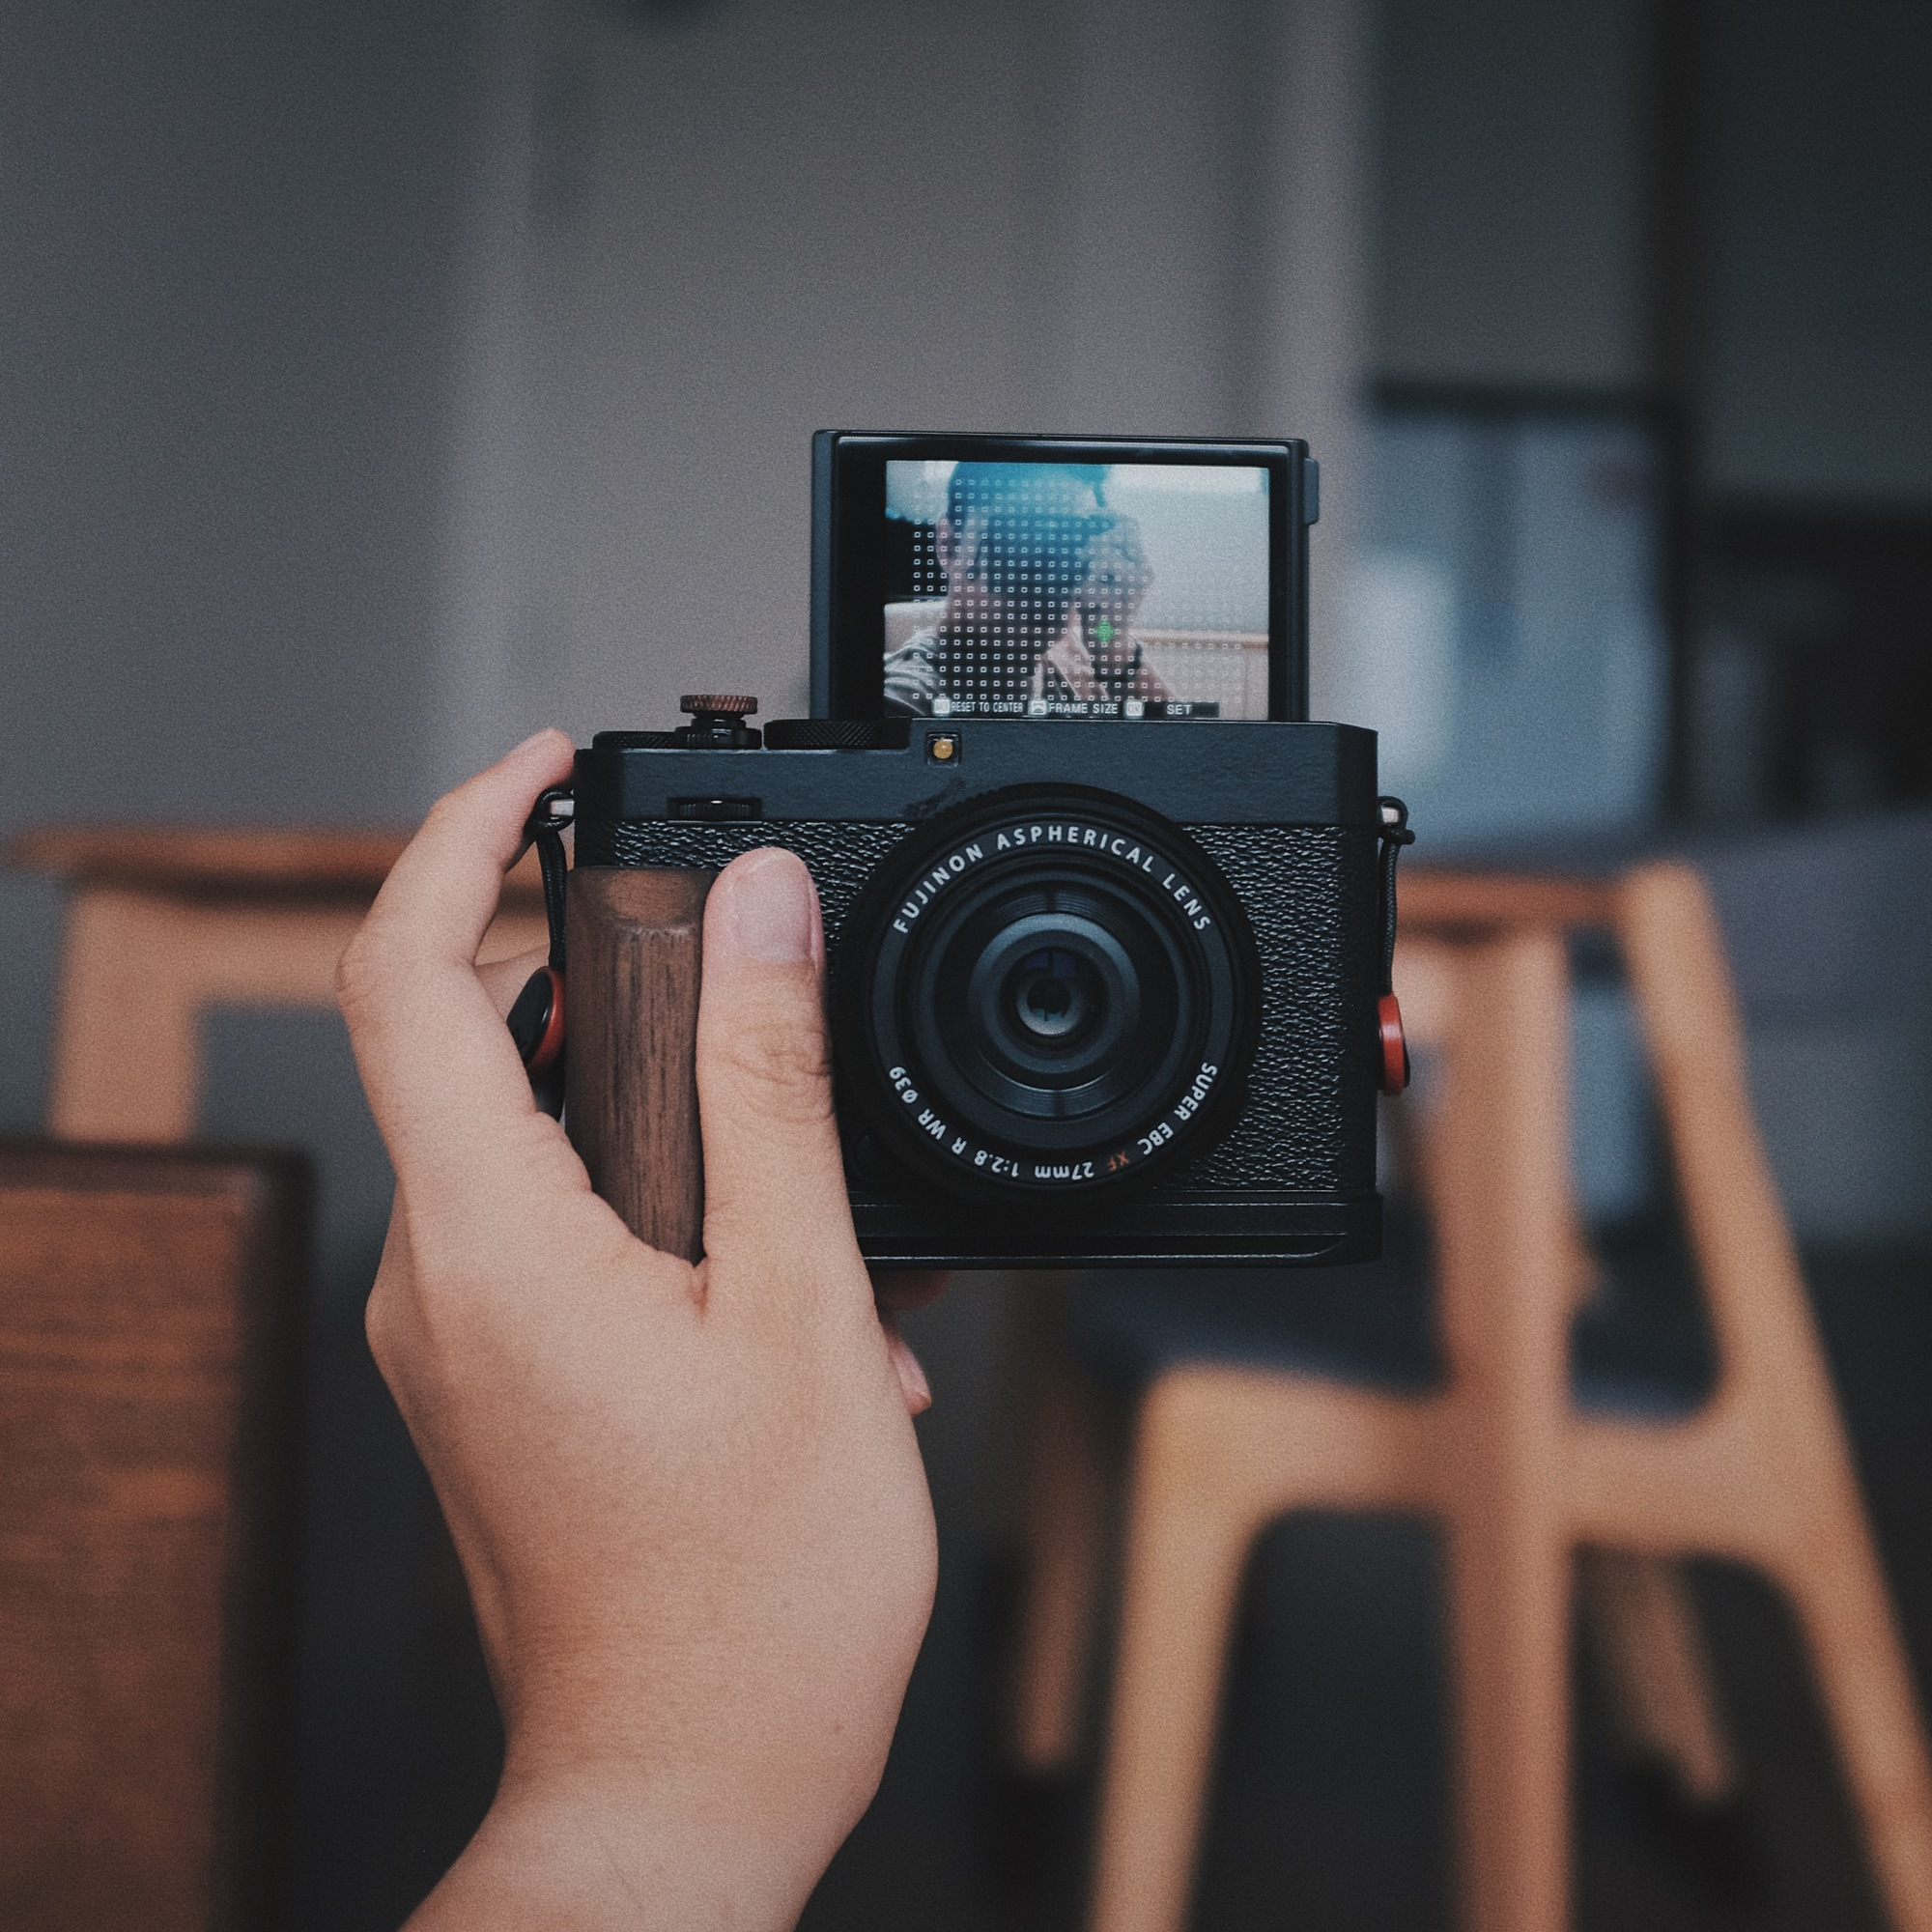
\includegraphics[width=\linewidth]{\envfinaldir/coverpic-prod.jpg}\par
            % \vskip 30pt
            \vfill

            \normalsize\rmfamily\scshape
            \copyright{} The Web Digest Project \hfill\large \envdatestr
        \end{center}
    \end{titlepage}
    % \restoregeometry
}
\newcommand{\simplehref}[1]{%
    \textcolor{blue!80!green}{\href{#1}{#1}}%
}
\renewcommand{\contentsname}{\center\Huge\sffamily\bfseries Contents\par\vskip 20pt}
\newcounter{ipartcounter}
\setcounter{ipartcounter}{0}
\newcommand{\ipart}[1]{
    % \vskip 20pt
    \clearpage
    \stepcounter{ipartcounter}
    \phantomsection
    \addcontentsline{toc}{chapter}{#1}
    % \begin{center}
    %     \Huge
    %     \sffamily\bfseries
    %     #1
    % \end{center}
    % \vskip 20pt plus 7pt
}
\newcounter{ichaptercounter}
\setcounter{ichaptercounter}{0}
\newcommand{\ichapter}[1]{
    % \vskip 20pt
    \clearpage
    \stepcounter{ichaptercounter}
    \phantomsection
    \addcontentsline{toc}{section}{\numberline{\arabic{ichaptercounter}}#1}
    \begin{center}
        \Huge
        \sffamily\bfseries
        #1
    \end{center}
    \vskip 20pt plus 7pt
}
\newcommand{\entrytitlefont}[1]{\subsection*{\raggedright\Large\sffamily\bfseries#1}}
\newcommand{\entryitemGeneric}[2]{
    % argv: title, url
    \parbox{\linewidth}{
        \entrytitlefont{#1}\par\vskip 5pt
        \footnotesize\ttfamily\mdseries
        \simplehref{#2}
    }\vskip 11pt plus 11pt minus 1pt
}
\newcommand{\entryitemGithub}[3]{
    % argv: title, url, desc
    \parbox{\linewidth}{
        \entrytitlefont{#1}\par\vskip 5pt
        \footnotesize\ttfamily\mdseries
        \simplehref{#2}\par\vskip 5pt
        \small\rmfamily\mdseries#3
    }\vskip 11pt plus 11pt minus 1pt
}
\newcommand{\entryitemAp}[3]{
    % argv: title, url, desc
    \parbox{\linewidth}{
        \entrytitlefont{#1}\par\vskip 5pt
        \footnotesize\ttfamily\mdseries
        \simplehref{#2}\par\vskip 5pt
        \small\rmfamily\mdseries#3
    }\vskip 11pt plus 11pt minus 1pt
}
\newcommand{\entryitemHackernews}[3]{
    % argv: title, hnurl, rawurl
    % \parbox{\linewidth}{
    %     \entrytitlefont{#1}\par\vskip 5pt
    %     \footnotesize\ttfamily\mdseries
    %     \simplehref{#3}\par
    %     \textcolor{black!50}{\href{#2}{#2}}
    % }\vskip 11pt plus 11pt minus 1pt
    \begin{minipage}{\linewidth}
            \entrytitlefont{#1}\par\vskip 5pt
            \footnotesize\ttfamily\mdseries
            \simplehref{#3}\par
            \textcolor{black!50}{\href{#2}{#2}}
    \end{minipage}\par\vskip 11pt plus 11pt minus 1pt
}







\begin{document}

\makeheader

\tableofcontents\clearpage




\ipart{Developers}
\ichapter{Hacker News}
\entryitemTwoLinks{Evaluating the impact of AI on the labor market: Current state of affairs}{https://news.ycombinator.com/item?id=45442743}{https://budgetlab.yale.edu/research/evaluating-impact-ai-labor-market-current-state-affairs}

\entryitemTwoLinks{U.S. Lost 32,000 Private-Sector Jobs in September, Says Payroll Processor}{https://news.ycombinator.com/item?id=45442185}{https://www.wsj.com/economy/jobs/u-s-lost-32-000-jobs-in-september-says-payroll-processor-06528340}

\entryitemTwoLinks{ICE Is Buying a Tool to Track Phones, Without Warrants}{https://news.ycombinator.com/item?id=45441983}{https://olgalautman.substack.com/p/ice-is-buying-a-tool-to-track-hundreds}

\entryitemTwoLinks{Jane Goodall has died}{https://news.ycombinator.com/item?id=45441069}{https://www.latimes.com/obituaries/story/2025-10-01/jane-goodall-chimpanzees-dead}

\entryitemTwoLinks{What good workplace politics looks like in practice}{https://news.ycombinator.com/item?id=45440571}{https://terriblesoftware.org/2025/10/01/stop-avoiding-politics/}

\entryitemTwoLinks{OpenTSLM: Language models that understand time series}{https://news.ycombinator.com/item?id=45440431}{https://www.opentslm.com/}

\entryitemTwoLinks{Solar leads EU electricity generation as renewables hit 54\%}{https://news.ycombinator.com/item?id=45440387}{https://electrek.co/2025/09/30/solar-leads-eu-electricity-generation-as-renewables-hit-54-percent/}

\entryitemTwoLinks{Codeberg Reaches 300k Projects}{https://news.ycombinator.com/item?id=45439955}{https://codeberg.org/}

\entryitemTwoLinks{DuckDuckGo Donates \$25,000 to The Perl and Raku Foundation v2025}{https://news.ycombinator.com/item?id=45439883}{https://www.perl.com/article/duckduckgo-donates-25-000-to-the-perl-and-raku-foundation-v2025/}

\entryitemTwoLinks{No more "check mail from other accounts" in Gmail web}{https://news.ycombinator.com/item?id=45439670}{https://support.google.com/mail/answer/16604719?hl=en}

\entryitemTwoLinks{Ask HN: Who is hiring? (October 2025)}{https://news.ycombinator.com/item?id=45438503}{https://news.ycombinator.com/item?id=45438503}

\entryitemTwoLinks{Building the heap: racking 30 petabytes of hard drives for pretraining}{https://news.ycombinator.com/item?id=45438496}{https://si.inc/posts/the-heap/}

\entryitemTwoLinks{Show HN: Autism Simulator}{https://news.ycombinator.com/item?id=45438346}{https://autism-simulator.vercel.app/}

\entryitemTwoLinks{Unix philosophy and filesystem access makes Claude Code amazing}{https://news.ycombinator.com/item?id=45437893}{https://www.alephic.com/writing/the-magic-of-claude-code}

\entryitemTwoLinks{Cursor 1.7}{https://news.ycombinator.com/item?id=45437735}{https://cursor.com/changelog/1-7}

\entryitemTwoLinks{Show HN: ChartDB Agent – Cursor for DB schema design}{https://news.ycombinator.com/item?id=45437594}{https://app.chartdb.io/ai}

\entryitemTwoLinks{Minimal files and config for a PWA}{https://news.ycombinator.com/item?id=45437326}{https://github.com/chr15m/minimal-pwa}

\entryitemTwoLinks{Detect Electron apps on Mac that hasn't been updated to fix the system wide lag}{https://news.ycombinator.com/item?id=45437112}{https://gist.github.com/tkafka/e3eb63a5ec448e9be6701bfd1f1b1e58}

\entryitemTwoLinks{TigerBeetle is a most interesting database}{https://news.ycombinator.com/item?id=45436534}{https://www.amplifypartners.com/blog-posts/why-tigerbeetle-is-the-most-interesting-database-in-the-world}

\entryitemTwoLinks{Our efforts, in part, define us}{https://news.ycombinator.com/item?id=45435825}{https://weakty.com/posts/efforts/}\ichapter{Phoronix}
\entryitemGeneric{\hskip 0pt{}TrueNAS 25.10-RC1 Brings Better Disk Import/Export, ZFS Rewrite Improvements}{https://www.phoronix.com/news/TrueNAS-25.10-RC1-Released}

\entryitemGeneric{\hskip 0pt{}A Minor Optimization Comes For x86 Memory Management In Linux 6.18}{https://www.phoronix.com/news/Linux-6.18-x86-mm}

\entryitemGeneric{\hskip 0pt{}Attack Vector Controls Can Now Manage VMSCAPE Mitigation}{https://www.phoronix.com/news/Linux-6.18-AVC-VMSCAPE}

\entryitemGeneric{\hskip 0pt{}More ASUS Motherboards Will Have Working Sensor Monitoring With Linux 6.18}{https://www.phoronix.com/news/Linux-6.18-HWMON}

\entryitemGeneric{\hskip 0pt{}Intel Arc Pro B50, Raspberry Pi 500+, Strix Halo \& Other September Highlights}{https://www.phoronix.com/news/September-2025}

\entryitemGeneric{\hskip 0pt{}EXT4, EROFS \& NTFS3 File-System Drivers Ready With Improvements For Linux 6.18}{https://www.phoronix.com/news/Linux-6.18-EXT4-EROFS-NTFS3}

\entryitemGeneric{\hskip 0pt{}openSUSE Leap 16 Released - Requires x86-64-v2 CPUs, No x86 32-bit Support By Default}{https://www.phoronix.com/news/openSUSE-Leap-16}

\entryitemGeneric{\hskip 0pt{}Linus Torvalds Lashes Out At RISC-V Big Endian Plans}{https://www.phoronix.com/news/Torvalds-No-RISC-V-BE}

\entryitemGeneric{\hskip 0pt{}Academy Software Foundation's OpenColorIO Adds Vulkan Support}{https://www.phoronix.com/news/OpenColorIO-Adds-Vulkan}


\ipart{Developers~~~~(zh-Hans)}
\ichapter{Solidot}
\entryitemGeneric{\hskip 0pt{}Kindle Scribe 加入 AI 驱动的笔记本功能}{https://www.solidot.org/story?sid=82465}

\entryitemGeneric{\hskip 0pt{}Imgur 屏蔽英国用户访问}{https://www.solidot.org/story?sid=82464}

\entryitemGeneric{\hskip 0pt{}微软宣布 Windows 11 v25H2 GA}{https://www.solidot.org/story?sid=82463}

\entryitemGeneric{\hskip 0pt{}Cloudflare 赞助 Ladybird 浏览器引擎项目}{https://www.solidot.org/story?sid=82462}

\entryitemGeneric{\hskip 0pt{}阿富汗断网超过两天}{https://www.solidot.org/story?sid=82461}

\entryitemGeneric{\hskip 0pt{}Linus Torvalds 从 Linux 6.18 中完全移除了 Bcachefs }{https://www.solidot.org/story?sid=82460}

\entryitemGeneric{\hskip 0pt{}世界最高大桥花江峡谷大桥通车}{https://www.solidot.org/story?sid=82459}

\entryitemGeneric{\hskip 0pt{}CS 教授警告毕业生难找到工作}{https://www.solidot.org/story?sid=82458}

\entryitemGeneric{\hskip 0pt{}因 AI 需求大涨 DRAM 价格翻倍}{https://www.solidot.org/story?sid=82457}

\entryitemGeneric{\hskip 0pt{}微塑料可能削弱骨骼}{https://www.solidot.org/story?sid=82456}

\entryitemGeneric{\hskip 0pt{}阿富汗断网}{https://www.solidot.org/story?sid=82454}

\entryitemGeneric{\hskip 0pt{}投资财团以 550 亿美元私有化 EA}{https://www.solidot.org/story?sid=82453}

\entryitemGeneric{\hskip 0pt{}高糖芒果有助于降低糖尿病风险}{https://www.solidot.org/story?sid=82452}

\entryitemGeneric{\hskip 0pt{}日本公司研发出基于植物的生鱼片}{https://www.solidot.org/story?sid=82451}

\entryitemGeneric{\hskip 0pt{}RubyGems 社区发生项目控制权争夺战}{https://www.solidot.org/story?sid=82450}

\entryitemGeneric{\hskip 0pt{}加州公共和共享充电桩数量比加油站多 68\%}{https://www.solidot.org/story?sid=82449}

\entryitemGeneric{\hskip 0pt{}流浪行星发现有极光}{https://www.solidot.org/story?sid=82448}

\entryitemGeneric{\hskip 0pt{}瑞士周日公投以微弱多数批准电子身份证}{https://www.solidot.org/story?sid=82447}

\entryitemGeneric{\hskip 0pt{}F-Droid 发表声明反对 Google 验证应用开发者身份的要求}{https://www.solidot.org/story?sid=82446}

\entryitemGeneric{\hskip 0pt{}Linux 6.17 释出}{https://www.solidot.org/story?sid=82444}\ichapter{V2EX}
\entryitemGeneric{\hskip 0pt{}[宽带症候群] 上海联通离谱限速 5M}{https://www.v2ex.com/t/1163108}

\entryitemGeneric{\hskip 0pt{}[Apple] macos26 Preview 预览 BUG 求助}{https://www.v2ex.com/t/1163107}

\entryitemGeneric{\hskip 0pt{}[加密货币] 什么交易所可以 p2p 外币}{https://www.v2ex.com/t/1163106}

\entryitemGeneric{\hskip 0pt{}[分享创造] 欢迎来领 sora 2 的邀请码,也欢迎来这里分分享您的邀请码}{https://www.v2ex.com/t/1163105}

\entryitemGeneric{\hskip 0pt{}[Claude] Claude Code 再次大幅度提价}{https://www.v2ex.com/t/1163104}

\entryitemGeneric{\hskip 0pt{}[问与答] 撒尿时排出了一块直径在 10-12mm 的结石,兄弟们平时一定要注意合理饮食和运动啊}{https://www.v2ex.com/t/1163103}

\entryitemGeneric{\hskip 0pt{}[生活] 半夜刷户子的切片睡不着,起来 BB 两句}{https://www.v2ex.com/t/1163102}

\entryitemGeneric{\hskip 0pt{}[问与答] 户晨风到底是什么样的人?}{https://www.v2ex.com/t/1163101}

\entryitemGeneric{\hskip 0pt{}[问与答] 搞了个新站点 sora2video,想生成 sora2 视频的来试试吧,我搞了个 20\%的优惠券给 v 友}{https://www.v2ex.com/t/1163100}

\entryitemGeneric{\hskip 0pt{}[分享创造] 连夜肝出 Sora2,给大家品鉴一下, Nanobanana + Sora2 一站式体验}{https://www.v2ex.com/t/1163099}

\entryitemGeneric{\hskip 0pt{}[程序员] gemini 和 claude 体验对比}{https://www.v2ex.com/t/1163098}

\entryitemGeneric{\hskip 0pt{}[问与答] 现在感觉没有生孩子的必要了,有同感的吗}{https://www.v2ex.com/t/1163097}

\entryitemGeneric{\hskip 0pt{}[分享创造] 简陋的开发了一个 Sora2 的站点}{https://www.v2ex.com/t/1163096}

\entryitemGeneric{\hskip 0pt{}[问与答] 闲鱼购买虚拟卡券真的风险太大了,不如 pdd}{https://www.v2ex.com/t/1163094}

\entryitemGeneric{\hskip 0pt{}[MacBook Pro] 新旧 MacBook 数据迁移,迁移助理显示成功实际失败,最终还是 time machine 解决问题}{https://www.v2ex.com/t/1163093}

\entryitemGeneric{\hskip 0pt{}[分享发现] 真的被 glm 坑到了}{https://www.v2ex.com/t/1163091}

\entryitemGeneric{\hskip 0pt{}[宽带症候群] [求助]路由器上安装 homebox,跨运营商能跑满速度,用 webdav 读文件就被限速几百 KB/s}{https://www.v2ex.com/t/1163090}

\entryitemGeneric{\hskip 0pt{}[酷工作] 有木有在广州的 Flutter,可以短期四个月驻场开发的,需要 Flutter 两名 。工作地点在广州番禺市桥附近。}{https://www.v2ex.com/t/1163085}

\entryitemGeneric{\hskip 0pt{}[问与答] 想吃点好的,求推荐能秒开 TG 和油管 4K 的 VPS,月付 100 内~}{https://www.v2ex.com/t/1163084}

\entryitemGeneric{\hskip 0pt{}[分享创造] awesome sora2 prompt}{https://www.v2ex.com/t/1163083}

\entryitemGeneric{\hskip 0pt{}[问与答] 最近开始整治视频平台的真话类视频了?}{https://www.v2ex.com/t/1163081}

\entryitemGeneric{\hskip 0pt{}[Apple] 外置硬盘 Macos 系统升级提示无权限怎么办?}{https://www.v2ex.com/t/1163080}

\entryitemGeneric{\hskip 0pt{}[iPhone] 无人值守的 iPhone 有没有远程 ipkvm 的方案}{https://www.v2ex.com/t/1163079}

\entryitemGeneric{\hskip 0pt{}[分享创造] 做了个小工具,你一定用得到。}{https://www.v2ex.com/t/1163077}

\entryitemGeneric{\hskip 0pt{}[程序员] 一款 100\%基于 AI 大模型口述完成开发的 Chrome 实用插件,多设备共用一个 Chrome ID 想法记录好工具}{https://www.v2ex.com/t/1163076}

\entryitemGeneric{\hskip 0pt{}[Android] vivo 有点奇葩}{https://www.v2ex.com/t/1163075}

\entryitemGeneric{\hskip 0pt{}[健康] 码农日常应如何保护眼睛、颈椎,肩膀,腰,膀胱等无原厂换新的零部件?}{https://www.v2ex.com/t/1163074}

\entryitemGeneric{\hskip 0pt{}[Duolingo] 美区账号怎样才能加国区账号好友}{https://www.v2ex.com/t/1163073}

\entryitemGeneric{\hskip 0pt{}[ThinkPad] thinkpad t14s gen4 可以连接 Apple Display Monitor 吗}{https://www.v2ex.com/t/1163071}

\entryitemGeneric{\hskip 0pt{}[宽带症候群] 宽带下行莫名被降速到 1M}{https://www.v2ex.com/t/1163070}

\entryitemGeneric{\hskip 0pt{}[求职] 杭州,找远程兼职}{https://www.v2ex.com/t/1163069}

\entryitemGeneric{\hskip 0pt{}[推广] Openai 最新的视频生成模型 Sora2,旗舰视频和音频生成模型。}{https://www.v2ex.com/t/1163068}

\entryitemGeneric{\hskip 0pt{}[推广] 他来了他来了! Openai Sora2 发布了,你们都等了多久?}{https://www.v2ex.com/t/1163067}

\entryitemGeneric{\hskip 0pt{}[反馈] 屏蔽一下 HDR 炸弹头像!}{https://www.v2ex.com/t/1163065}

\entryitemGeneric{\hskip 0pt{}[推广] MK 机场 · 国庆特惠}{https://www.v2ex.com/t/1163064}

\entryitemGeneric{\hskip 0pt{}[问与答] 有没有人用过 oppo 的 o+互联 mac 版?是我的 MacBook 问题还是 o+互联本身的问题?}{https://www.v2ex.com/t/1163062}

\entryitemGeneric{\hskip 0pt{}[问与答] 求 1password 拼车,另外, 1p 拼车有风险吗?有无更好的解决办法?}{https://www.v2ex.com/t/1163061}

\entryitemGeneric{\hskip 0pt{}[问与答] 欧易平台与 hgkuou.com 到底是什么关系?}{https://www.v2ex.com/t/1163057}

\entryitemGeneric{\hskip 0pt{}[宽带症候群] 上海联通双节套餐加量 9929 限量}{https://www.v2ex.com/t/1163056}

\entryitemGeneric{\hskip 0pt{}[Android] 国内哪个手机支持象 Pixel10 一样的背部磁吸 magsafe 充电宝?}{https://www.v2ex.com/t/1163055}

\entryitemGeneric{\hskip 0pt{}[推广] 上海联通十月双节套餐加送流量通话 9929 限量办理}{https://www.v2ex.com/t/1163053}

\entryitemGeneric{\hskip 0pt{}[加密货币] ibkr 关门了, 港卡入金加密货币的无损渠道还有么?}{https://www.v2ex.com/t/1163052}

\entryitemGeneric{\hskip 0pt{}[推广] solaen release Sora2 !}{https://www.v2ex.com/t/1163051}

\entryitemGeneric{\hskip 0pt{}[NAS] 使用 stun 暴露飞牛影视到公网}{https://www.v2ex.com/t/1163050}

\entryitemGeneric{\hskip 0pt{}[iOS] 現在有可用的去知乎評論里的廣告插件、腳本沒啊,以前的都不起作用了}{https://www.v2ex.com/t/1163049}

\entryitemGeneric{\hskip 0pt{}[日本] 本站日本 (IT) 相关讨论合订本}{https://www.v2ex.com/t/1163047}

\entryitemGeneric{\hskip 0pt{}[分享创造] 分享下自己运营的生活权益小程序,对接了多个优惠渠道。}{https://www.v2ex.com/t/1163046}

\entryitemGeneric{\hskip 0pt{}[Surge] surge 配置通过 atrust docker 实现内网和外网都可以访问}{https://www.v2ex.com/t/1163045}

\entryitemGeneric{\hskip 0pt{}[创业组队] 需要一位熟悉 AI 架构和数据库的大神}{https://www.v2ex.com/t/1163044}

\entryitemGeneric{\hskip 0pt{}[分享发现] 开放者独立博客大全迎国庆,收录技术博客了!欢迎提交!开放者独立博客大全|博客导航大全 blog.kaifangzhe.com}{https://www.v2ex.com/t/1163043}


\ipart{Generic News}







\clearpage
\leavevmode\vfill
\footnotesize

Copyright \copyright{} 2023-2025 Neruthes and other contributors.

This document is published with CC BY-NC-ND 4.0 license.

The entries listed in this newsletter may be copyrighted by their respective creators.

This newsletter is generated by the Web Digest project.

The newsletters are also delivered via Telegram channel \CJKunderline{\href{https://t.me/webdigestchannel}{https://t.me/webdigestchannel}}.\\
RSS feed is available at \CJKunderline{\href{https://webdigest.pages.dev/rss.xml}{https://webdigest.pages.dev/rss.xml}}.

This newsletter is available in PDF at
\CJKunderline{\href{https://webdigest.pages.dev/}{https://webdigest.pages.dev/}}.

The source code being used to generate this newsletter is available at\\
\CJKunderline{\href{https://github.com/neruthes/webdigest}{https://github.com/neruthes/webdigest}}.

This newsletter is also available in
\CJKunderline{\href{http://webdigest.pages.dev/readhtml/\envyear/WebDigest-20251002.html}{HTML}} and
\CJKunderline{\href{https://github.com/neruthes/webdigest/blob/master/markdown/\envyear/WebDigest-20251002.md}{Markdown}}.


\coverpic{https://unsplash.com/photos/canadian-passport-and-brown-leather-wallet-on-white-fabric-YX5iTm\_PPvg}{Olivier Collet}


\end{document}
